% Options for packages loaded elsewhere
\PassOptionsToPackage{unicode}{hyperref}
\PassOptionsToPackage{hyphens}{url}
%
\documentclass[
  english,
  man,floatsintext]{apa6}
\usepackage{lmodern}
\usepackage{amssymb,amsmath}
\usepackage{ifxetex,ifluatex}
\ifnum 0\ifxetex 1\fi\ifluatex 1\fi=0 % if pdftex
  \usepackage[T1]{fontenc}
  \usepackage[utf8]{inputenc}
  \usepackage{textcomp} % provide euro and other symbols
\else % if luatex or xetex
  \usepackage{unicode-math}
  \defaultfontfeatures{Scale=MatchLowercase}
  \defaultfontfeatures[\rmfamily]{Ligatures=TeX,Scale=1}
\fi
% Use upquote if available, for straight quotes in verbatim environments
\IfFileExists{upquote.sty}{\usepackage{upquote}}{}
\IfFileExists{microtype.sty}{% use microtype if available
  \usepackage[]{microtype}
  \UseMicrotypeSet[protrusion]{basicmath} % disable protrusion for tt fonts
}{}
\makeatletter
\@ifundefined{KOMAClassName}{% if non-KOMA class
  \IfFileExists{parskip.sty}{%
    \usepackage{parskip}
  }{% else
    \setlength{\parindent}{0pt}
    \setlength{\parskip}{6pt plus 2pt minus 1pt}}
}{% if KOMA class
  \KOMAoptions{parskip=half}}
\makeatother
\usepackage{xcolor}
\IfFileExists{xurl.sty}{\usepackage{xurl}}{} % add URL line breaks if available
\IfFileExists{bookmark.sty}{\usepackage{bookmark}}{\usepackage{hyperref}}
\hypersetup{
  pdftitle={GenSamp: RESULTS},
  pdfauthor={Gleb Furman1 \& James E. Pustejovsky1},
  pdflang={en-EN},
  hidelinks,
  pdfcreator={LaTeX via pandoc}}
\urlstyle{same} % disable monospaced font for URLs
\usepackage{graphicx,grffile}
\makeatletter
\def\maxwidth{\ifdim\Gin@nat@width>\linewidth\linewidth\else\Gin@nat@width\fi}
\def\maxheight{\ifdim\Gin@nat@height>\textheight\textheight\else\Gin@nat@height\fi}
\makeatother
% Scale images if necessary, so that they will not overflow the page
% margins by default, and it is still possible to overwrite the defaults
% using explicit options in \includegraphics[width, height, ...]{}
\setkeys{Gin}{width=\maxwidth,height=\maxheight,keepaspectratio}
% Set default figure placement to htbp
\makeatletter
\def\fps@figure{htbp}
\makeatother
\setlength{\emergencystretch}{3em} % prevent overfull lines
\providecommand{\tightlist}{%
  \setlength{\itemsep}{0pt}\setlength{\parskip}{0pt}}
\setcounter{secnumdepth}{-\maxdimen} % remove section numbering
% Make \paragraph and \subparagraph free-standing
\ifx\paragraph\undefined\else
  \let\oldparagraph\paragraph
  \renewcommand{\paragraph}[1]{\oldparagraph{#1}\mbox{}}
\fi
\ifx\subparagraph\undefined\else
  \let\oldsubparagraph\subparagraph
  \renewcommand{\subparagraph}[1]{\oldsubparagraph{#1}\mbox{}}
\fi
% Manuscript styling
\usepackage{upgreek}
\captionsetup{font=singlespacing,justification=justified}

% Table formatting
\usepackage{longtable}
\usepackage{lscape}
% \usepackage[counterclockwise]{rotating}   % Landscape page setup for large tables
\usepackage{multirow}		% Table styling
\usepackage{tabularx}		% Control Column width
\usepackage[flushleft]{threeparttable}	% Allows for three part tables with a specified notes section
\usepackage{threeparttablex}            % Lets threeparttable work with longtable

% Create new environments so endfloat can handle them
% \newenvironment{ltable}
%   {\begin{landscape}\begin{center}\begin{threeparttable}}
%   {\end{threeparttable}\end{center}\end{landscape}}
\newenvironment{lltable}{\begin{landscape}\begin{center}\begin{ThreePartTable}}{\end{ThreePartTable}\end{center}\end{landscape}}

% Enables adjusting longtable caption width to table width
% Solution found at http://golatex.de/longtable-mit-caption-so-breit-wie-die-tabelle-t15767.html
\makeatletter
\newcommand\LastLTentrywidth{1em}
\newlength\longtablewidth
\setlength{\longtablewidth}{1in}
\newcommand{\getlongtablewidth}{\begingroup \ifcsname LT@\roman{LT@tables}\endcsname \global\longtablewidth=0pt \renewcommand{\LT@entry}[2]{\global\advance\longtablewidth by ##2\relax\gdef\LastLTentrywidth{##2}}\@nameuse{LT@\roman{LT@tables}} \fi \endgroup}

% \setlength{\parindent}{0.5in}
% \setlength{\parskip}{0pt plus 0pt minus 0pt}

% \usepackage{etoolbox}
\makeatletter
\patchcmd{\HyOrg@maketitle}
  {\section{\normalfont\normalsize\abstractname}}
  {\section*{\normalfont\normalsize\abstractname}}
  {}{\typeout{Failed to patch abstract.}}
\patchcmd{\HyOrg@maketitle}
  {\section{\protect\normalfont{\@title}}}
  {\section*{\protect\normalfont{\@title}}}
  {}{\typeout{Failed to patch title.}}
\makeatother
\shorttitle{RESULTS}
\usepackage{csquotes}
\ifxetex
  % Load polyglossia as late as possible: uses bidi with RTL langages (e.g. Hebrew, Arabic)
  \usepackage{polyglossia}
  \setmainlanguage[]{english}
\else
  \usepackage[shorthands=off,main=english]{babel}
\fi

\title{GenSamp: RESULTS}
\author{Gleb Furman\textsuperscript{1} \& James E. Pustejovsky\textsuperscript{1}}
\date{}


\affiliation{\vspace{0.5cm}\textsuperscript{1} University of Texas at Austin}

\begin{document}
\maketitle

\hypertarget{setup}{%
\section{Setup}\label{setup}}

\hypertarget{packages-and-data}{%
\subsection{Packages and Data}\label{packages-and-data}}

\hypertarget{organize-objects}{%
\subsection{Organize Objects}\label{organize-objects}}

\begin{verbatim}
## Joining, by = "DSID"
\end{verbatim}

\begin{verbatim}
## Parsed with column specification:
## cols(
##   vnames = col_character(),
##   Variables = col_character(),
##   Sub = col_character(),
##   Category = col_character(),
##   Type = col_character()
## )
## Parsed with column specification:
## cols(
##   vnames = col_character(),
##   Variables = col_character(),
##   Sub = col_character(),
##   Category = col_character(),
##   Type = col_character()
## )
\end{verbatim}

\begin{verbatim}
## Joining, by = "vnames"
\end{verbatim}

\hypertarget{data-summary}{%
\section{Data Summary}\label{data-summary}}

\hypertarget{covaraite-statistics}{%
\subsection{Covaraite Statistics}\label{covaraite-statistics}}

\begin{verbatim}
## `summarise()` ungrouping output (override with `.groups` argument)
\end{verbatim}

\begin{verbatim}
## Joining, by = "vnames"
\end{verbatim}

\begin{verbatim}
## Joining, by = c("vnames", "Variables", "Sub", "Category", "Type")
\end{verbatim}

\hypertarget{continuous-variable-distributions}{%
\subsection{Continuous variable distributions}\label{continuous-variable-distributions}}

\begin{verbatim}
## Joining, by = "vnames"
\end{verbatim}

\begin{verbatim}
## `stat_bin()` using `bins = 30`. Pick better value with `binwidth`.
\end{verbatim}

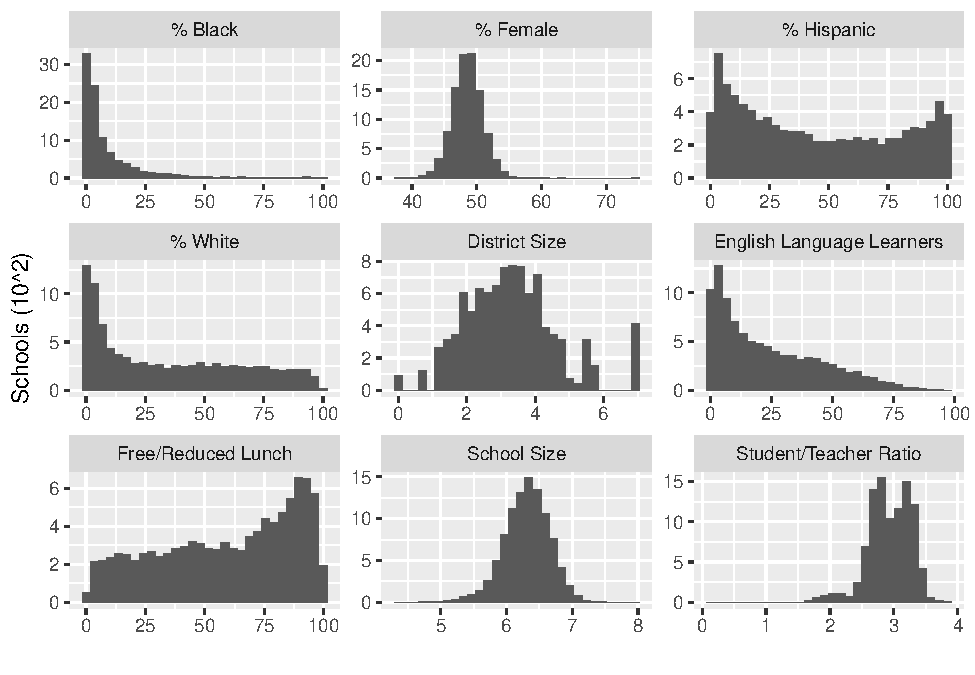
\includegraphics{5---Analysis_files/figure-latex/unnamed-chunk-2-1.pdf}

\hypertarget{methods-summary}{%
\section{Methods Summary}\label{methods-summary}}

\hypertarget{cluster-analysis}{%
\subsection{Cluster Analysis}\label{cluster-analysis}}

\hypertarget{selecting-k}{%
\subsubsection{Selecting k}\label{selecting-k}}

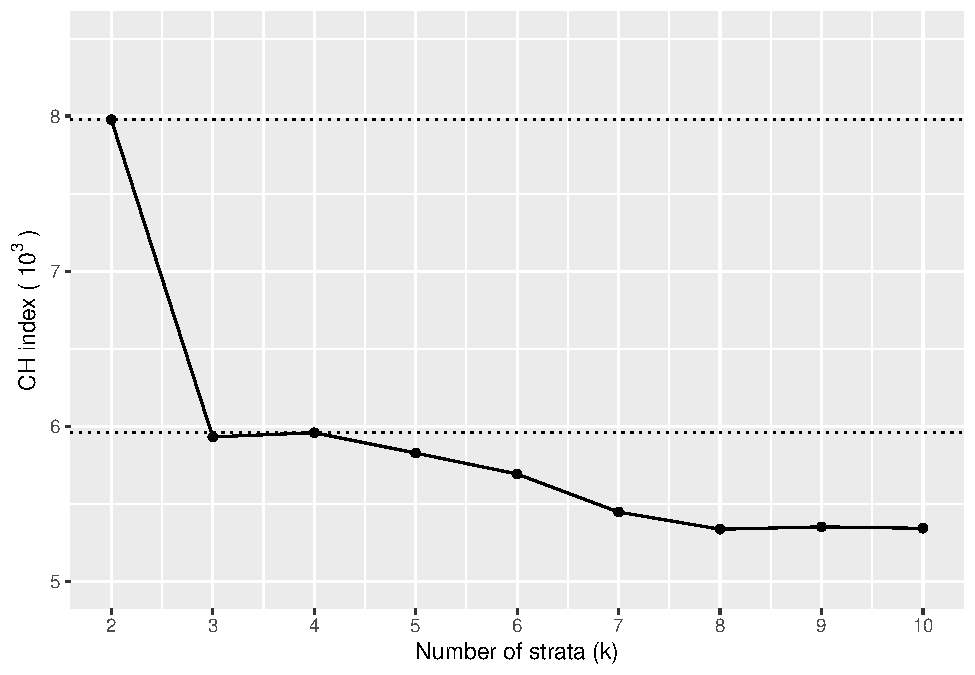
\includegraphics{5---Analysis_files/figure-latex/unnamed-chunk-3-1.pdf}

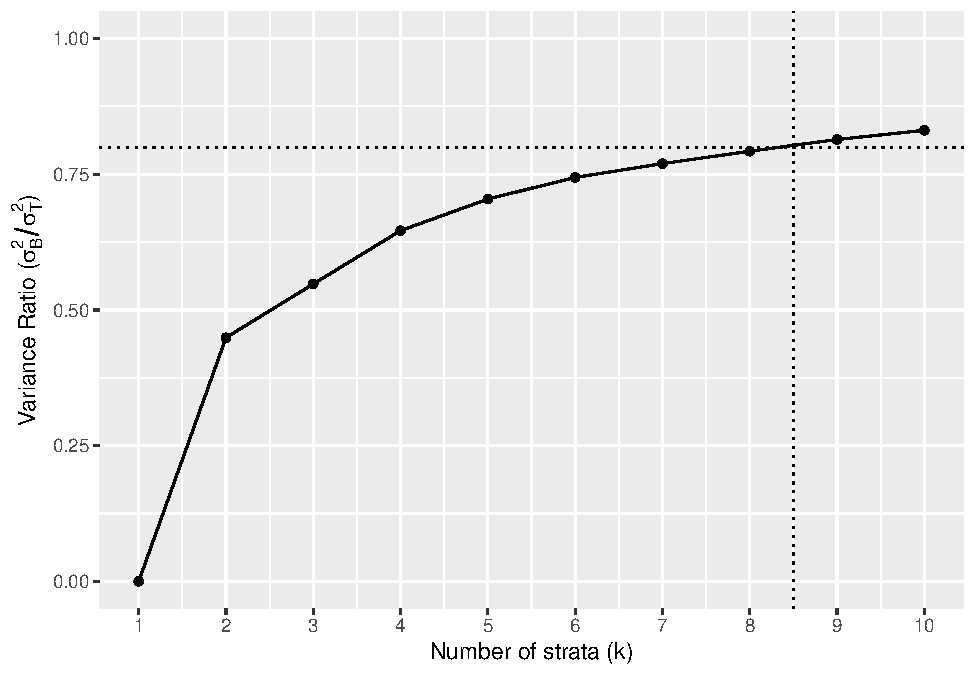
\includegraphics{5---Analysis_files/figure-latex/unnamed-chunk-4-1.pdf}

\begin{verbatim}
## `summarise()` regrouping output by 'k' (override with `.groups` argument)
\end{verbatim}

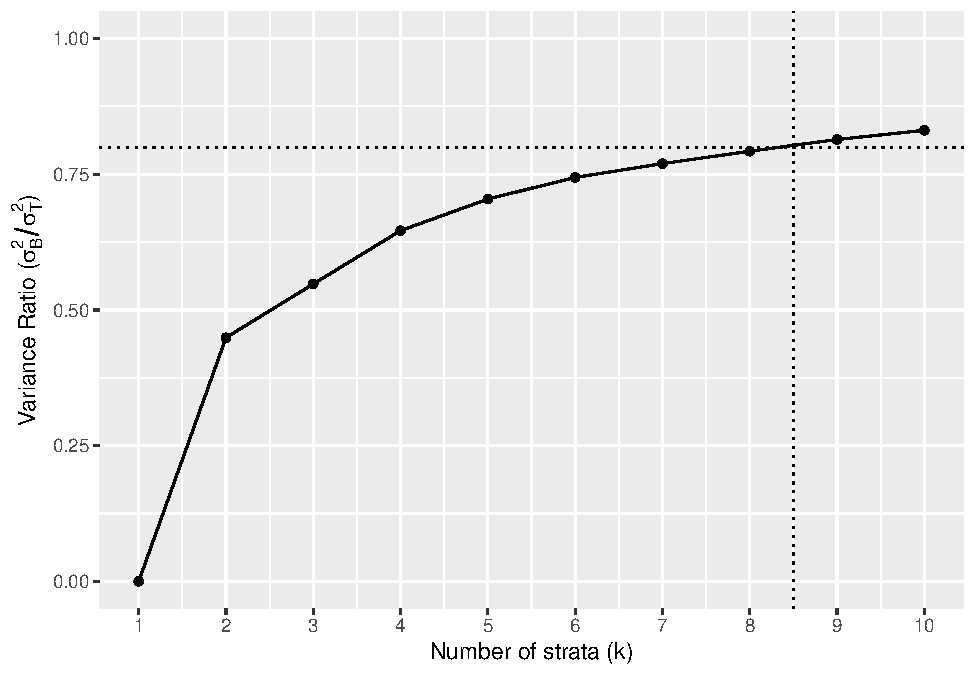
\includegraphics{5---Analysis_files/figure-latex/unnamed-chunk-5-1.pdf}

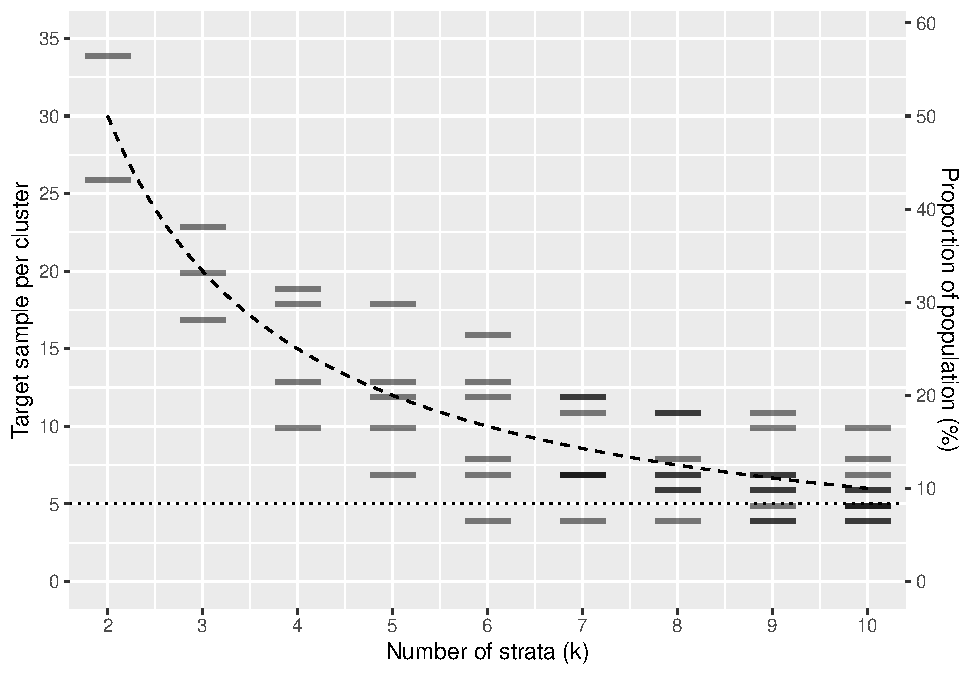
\includegraphics{5---Analysis_files/figure-latex/unnamed-chunk-6-1.pdf}

\begin{verbatim}
## `summarise()` regrouping output by 'strata' (override with `.groups` argument)
\end{verbatim}

\begin{verbatim}
## Joining, by = "var"
\end{verbatim}

\begin{verbatim}
## Joining, by = "vnames"
\end{verbatim}

\begin{verbatim}
## Warning: Using alpha for a discrete variable is not advised.
\end{verbatim}

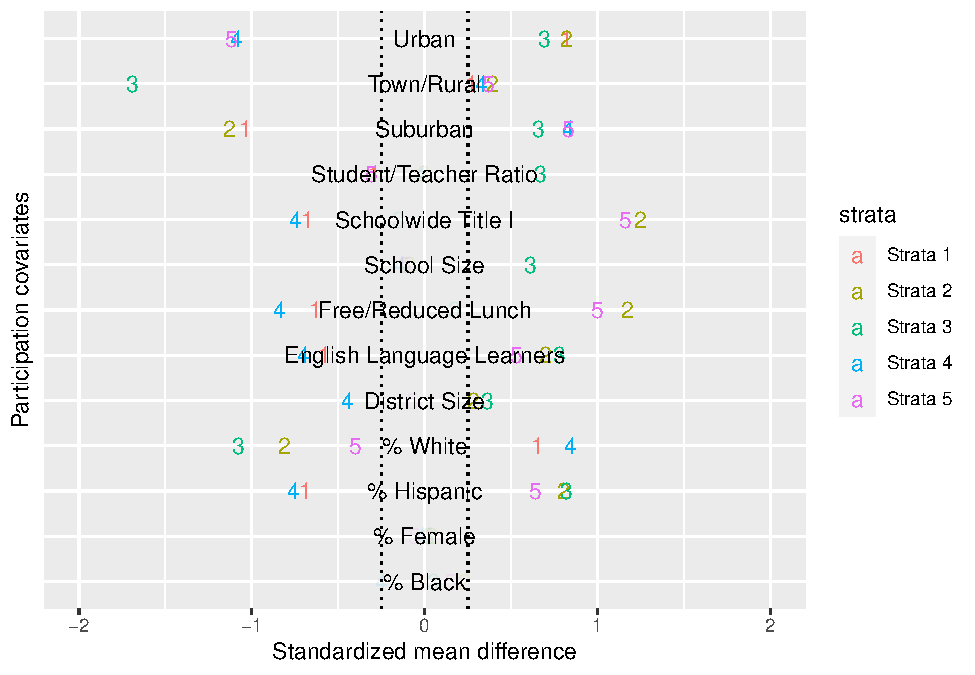
\includegraphics{5---Analysis_files/figure-latex/unnamed-chunk-8-1.pdf}

\begin{verbatim}
## Note: Using an external vector in selections is ambiguous.
## i Use `all_of(covariates)` instead of `covariates` to silence this message.
## i See <https://tidyselect.r-lib.org/reference/faq-external-vector.html>.
## This message is displayed once per session.
\end{verbatim}

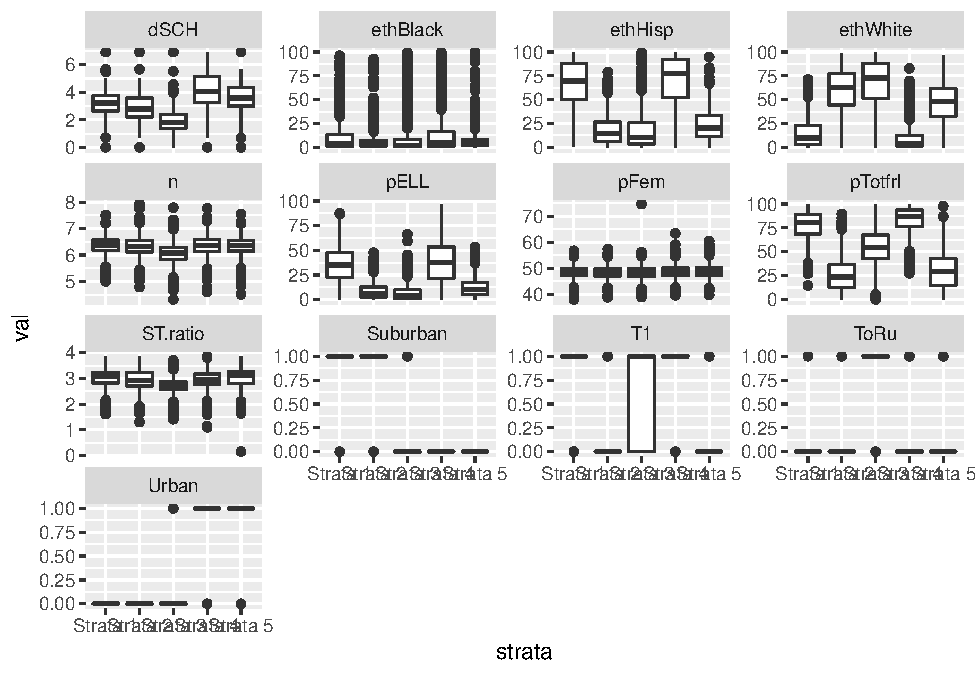
\includegraphics{5---Analysis_files/figure-latex/unnamed-chunk-9-1.pdf}

\hypertarget{participation-generating-model}{%
\subsection{Participation Generating Model}\label{participation-generating-model}}

\begin{table}[H]
\centering
\begin{tabular}{r|l|l|l|l}
\hline
log\_odds & Variables & Sub & Category & Type\\
\hline
0.019 & Schoolwide Title I & Status & School Data & Prop\\
\hline
0.374 & School Size & Enrollment & School Data & Mean\\
\hline
0.081 & Free/Reduced Lunch & Status & Student Data & Mean\\
\hline
0.433 & Urban & Urbanicity & School Data & Prop\\
\hline
0.007 & Suburban & Urbanicity & School Data & Prop\\
\hline
-0.403 & Town/Rural & Urbanicity & School Data & Prop\\
\hline
-0.538 & \% White & Ethnicity & Student Data & Mean\\
\hline
0.291 & \% Black & Ethnicity & Student Data & Mean\\
\hline
0.395 & \% Hispanic & Ethnicity & Student Data & Mean\\
\hline
-0.019 & \% Female & Gender & Student Data & Mean\\
\hline
-0.101 & Student/Teacher Ratio & Enrollment & School Data & Mean\\
\hline
0.520 & District Size & District & School Data & Mean\\
\hline
0.412 & English Language Learners & Status & Student Data & Mean\\
\hline
\end{tabular}
\end{table}

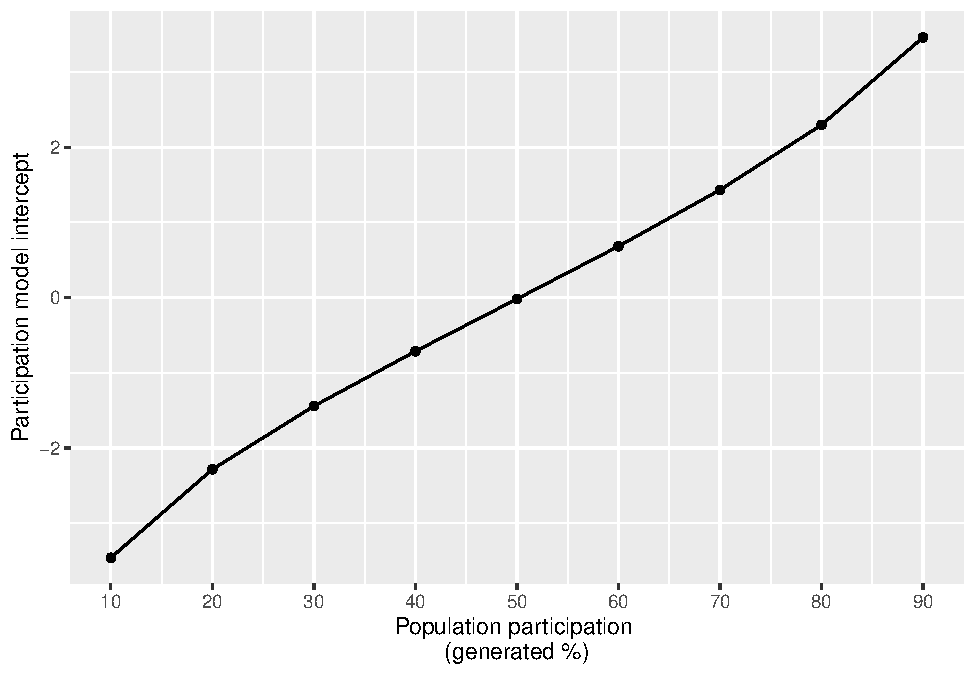
\includegraphics{5---Analysis_files/figure-latex/unnamed-chunk-11-1.pdf}

\begin{verbatim}
## `stat_bin()` using `bins = 30`. Pick better value with `binwidth`.
\end{verbatim}

\begin{figure}
\centering
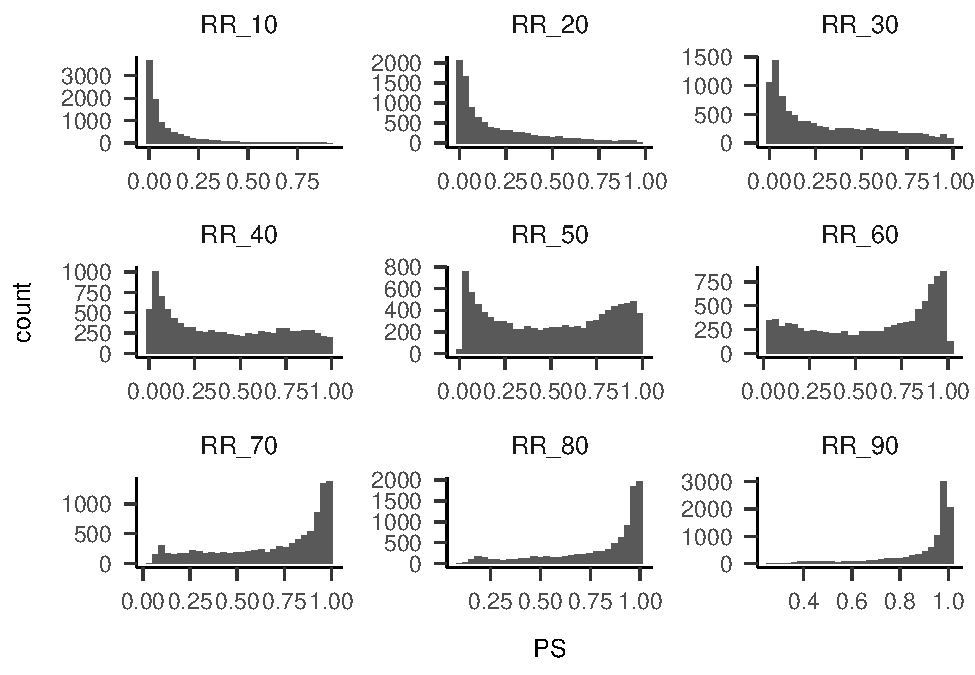
\includegraphics{5---Analysis_files/figure-latex/unnamed-chunk-12-1.pdf}
\caption{\label{fig:unnamed-chunk-12-1}Distributions of Participation Propensity Scores}
\end{figure}

\begin{verbatim}
## Joining, by = "DSID"
\end{verbatim}

\begin{figure}
\centering
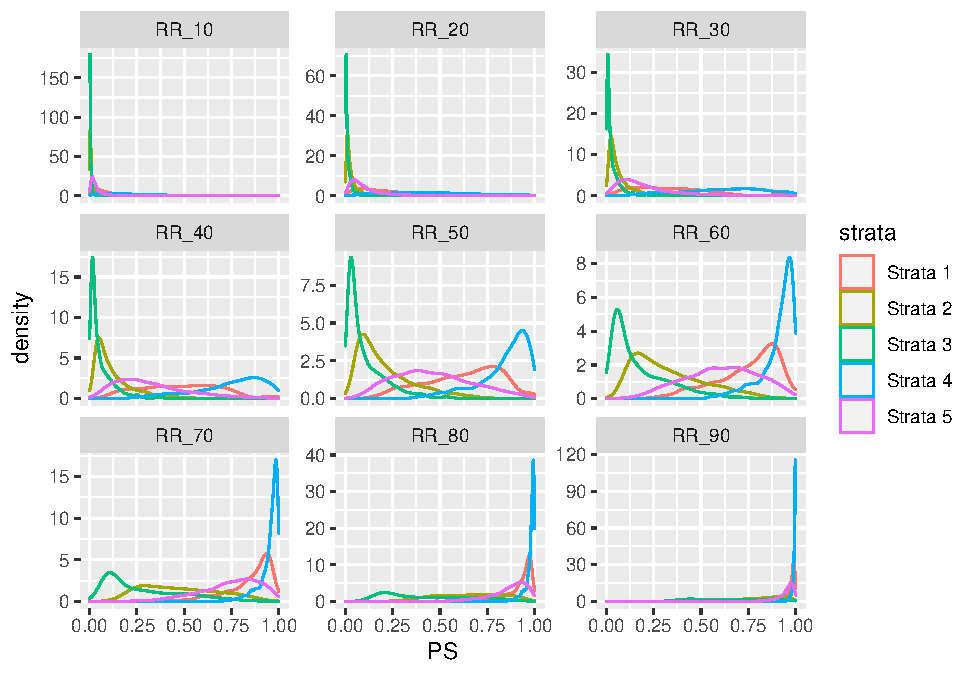
\includegraphics{5---Analysis_files/figure-latex/unnamed-chunk-12-2.pdf}
\caption{\label{fig:unnamed-chunk-12-2}Distributions of Participation Propensity Scores}
\end{figure}

\begin{verbatim}
## Joining, by = "DSID"
\end{verbatim}

\begin{figure}
\centering
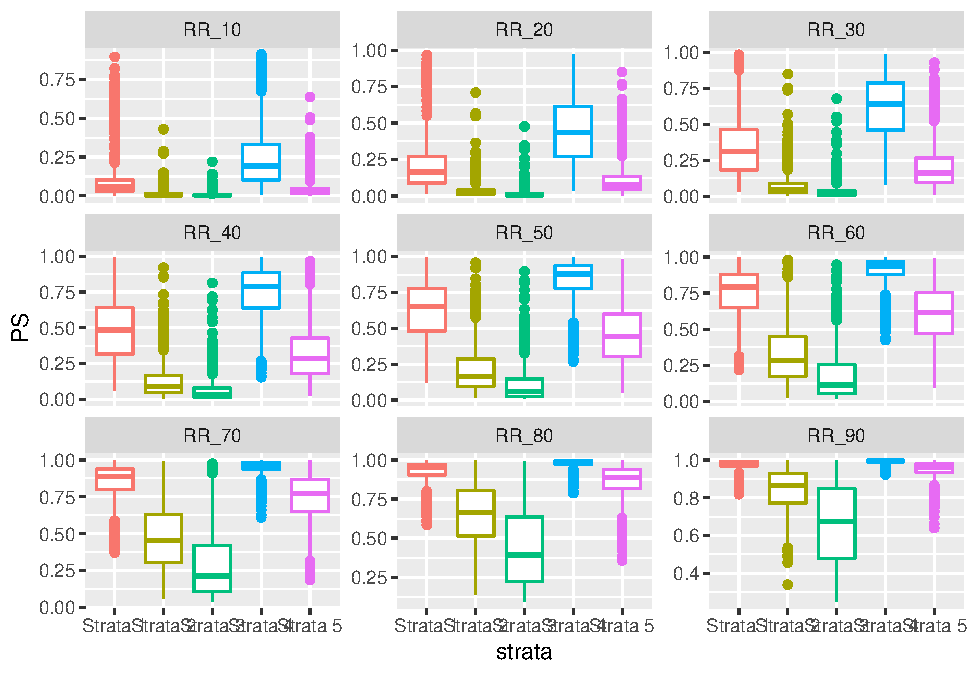
\includegraphics{5---Analysis_files/figure-latex/unnamed-chunk-12-3.pdf}
\caption{\label{fig:unnamed-chunk-12-3}Distributions of Participation Propensity Scores}
\end{figure}

\hypertarget{results}{%
\section{Results}\label{results}}

\hypertarget{generalizability}{%
\subsection{Generalizability}\label{generalizability}}

\hypertarget{b-index}{%
\subsubsection{B Index}\label{b-index}}

\begin{verbatim}
## `summarise()` regrouping output by 'sample_method', 'RR', 'Clustering' (override with `.groups` argument)
\end{verbatim}

\begin{figure}
\centering
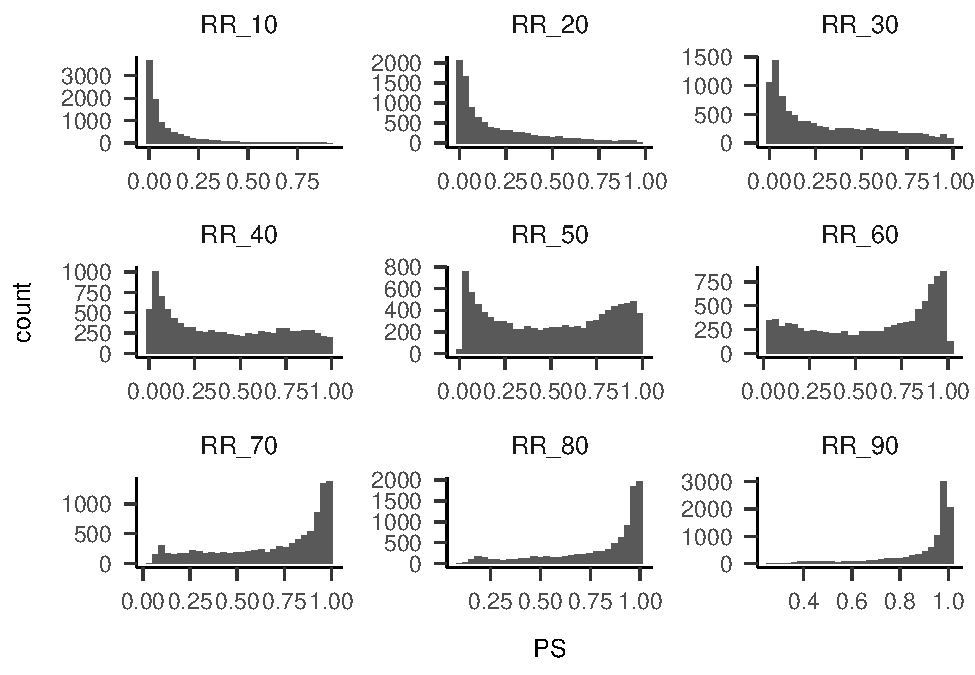
\includegraphics{5---Analysis_files/figure-latex/unnamed-chunk-13-1.pdf}
\caption{\label{fig:unnamed-chunk-13}Averge B-Index}
\end{figure}

\hypertarget{standardized-mean-differences}{%
\subsubsection{Standardized mean differences}\label{standardized-mean-differences}}

\begin{verbatim}
## Joining, by = "var"
\end{verbatim}

\begin{verbatim}
## `summarise()` regrouping output by 'sample_method', 'RR', 'var', 'Sampling' (override with `.groups` argument)
\end{verbatim}

\begin{verbatim}
## Joining, by = "vnames"
## Joining, by = "vnames"
\end{verbatim}

\begin{figure}
\centering
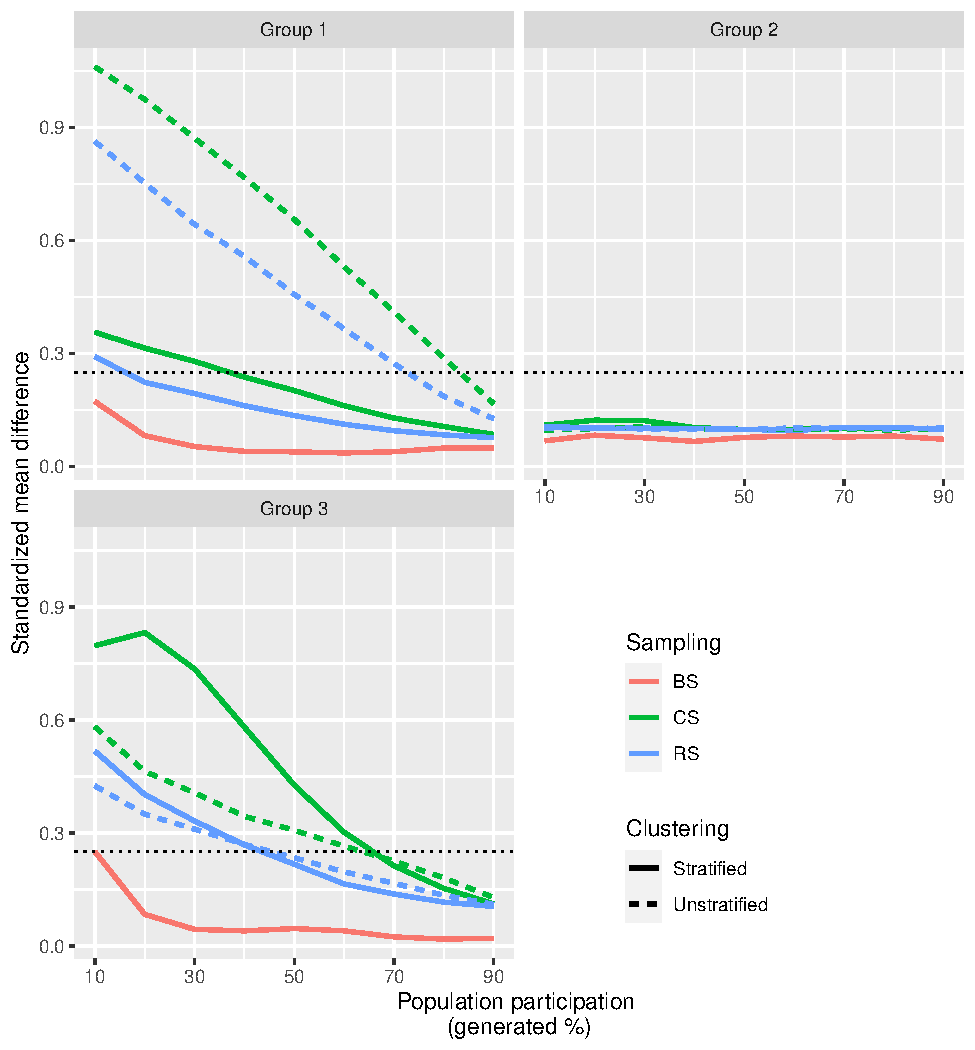
\includegraphics{5---Analysis_files/figure-latex/unnamed-chunk-14-1.pdf}
\caption{\label{fig:unnamed-chunk-14}Average SMDs}
\end{figure}

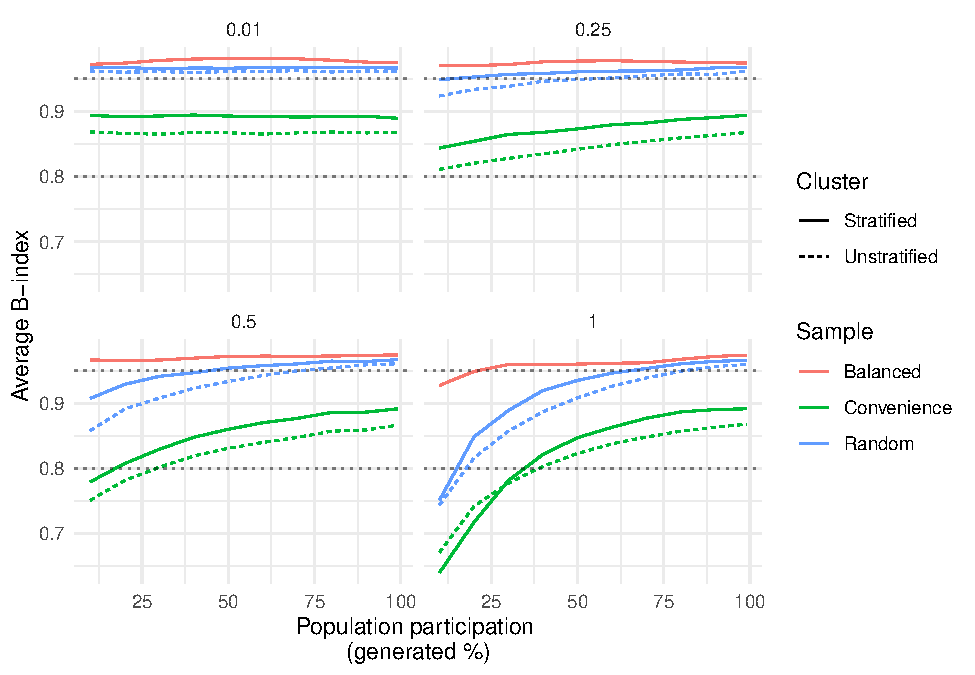
\includegraphics{5---Analysis_files/figure-latex/unnamed-chunk-15-1.pdf}

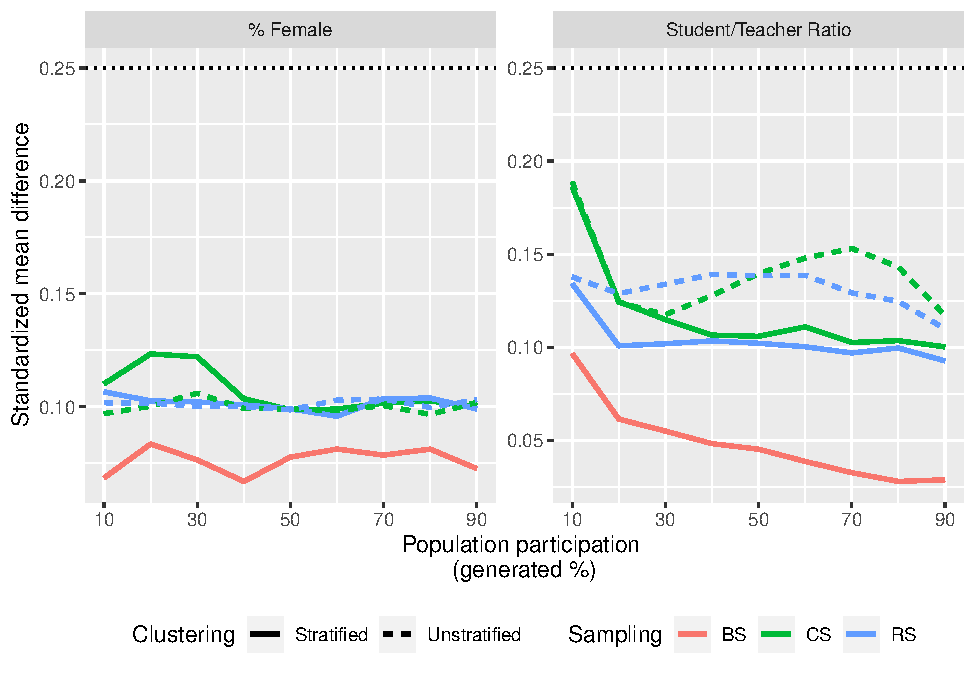
\includegraphics{5---Analysis_files/figure-latex/unnamed-chunk-16-1.pdf}
\#\#\# Examples for presentations

\hypertarget{v-ratio-and-log-odds}{%
\subsubsection{V-ratio and Log odds}\label{v-ratio-and-log-odds}}

\begin{verbatim}
## `summarise()` regrouping output by 'vnames', 'T.SS' (override with `.groups` argument)
\end{verbatim}

\begin{verbatim}
## `summarise()` regrouping output by 'vnames' (override with `.groups` argument)
\end{verbatim}

\begin{verbatim}
## Joining, by = "vnames"
## Joining, by = "vnames"
\end{verbatim}

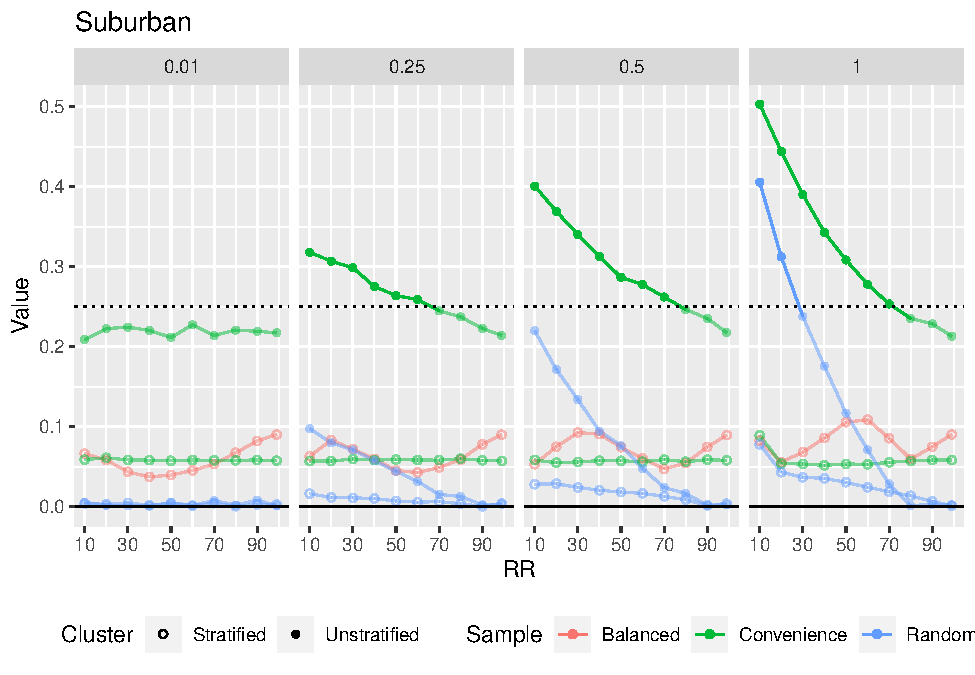
\includegraphics{5---Analysis_files/figure-latex/unnamed-chunk-18-1.pdf}

\hypertarget{test}{%
\subsubsection{Test}\label{test}}

\begin{verbatim}
## Joining, by = c("vnames", "log_odds")
\end{verbatim}

\begin{verbatim}
## `geom_smooth()` using formula 'y ~ x'
\end{verbatim}

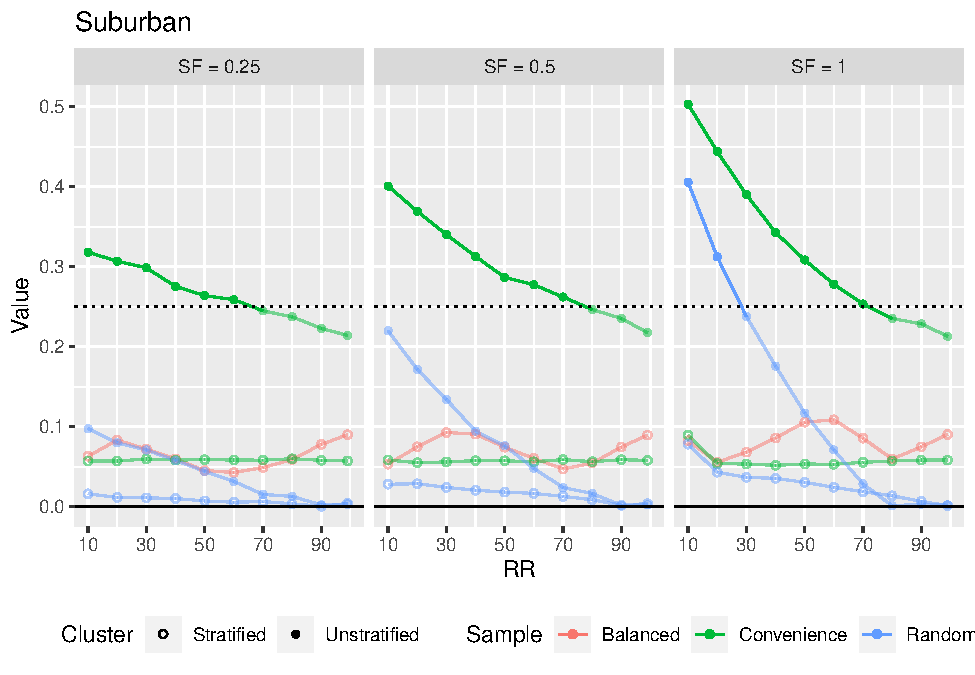
\includegraphics{5---Analysis_files/figure-latex/unnamed-chunk-20-1.pdf}

\begin{verbatim}
## `geom_smooth()` using formula 'y ~ x'
\end{verbatim}

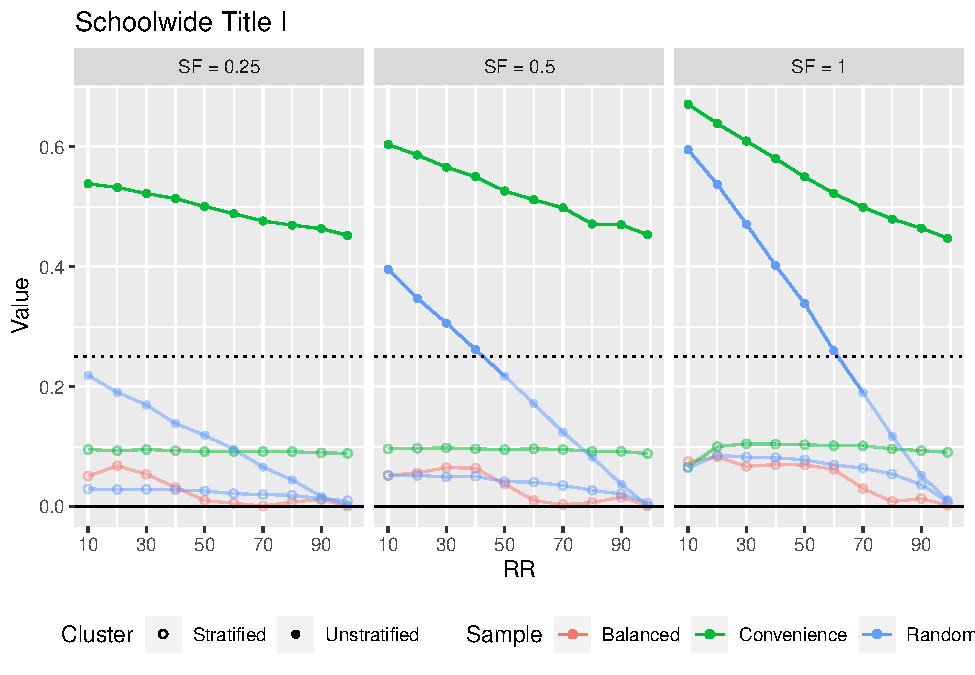
\includegraphics{5---Analysis_files/figure-latex/unnamed-chunk-20-2.pdf}

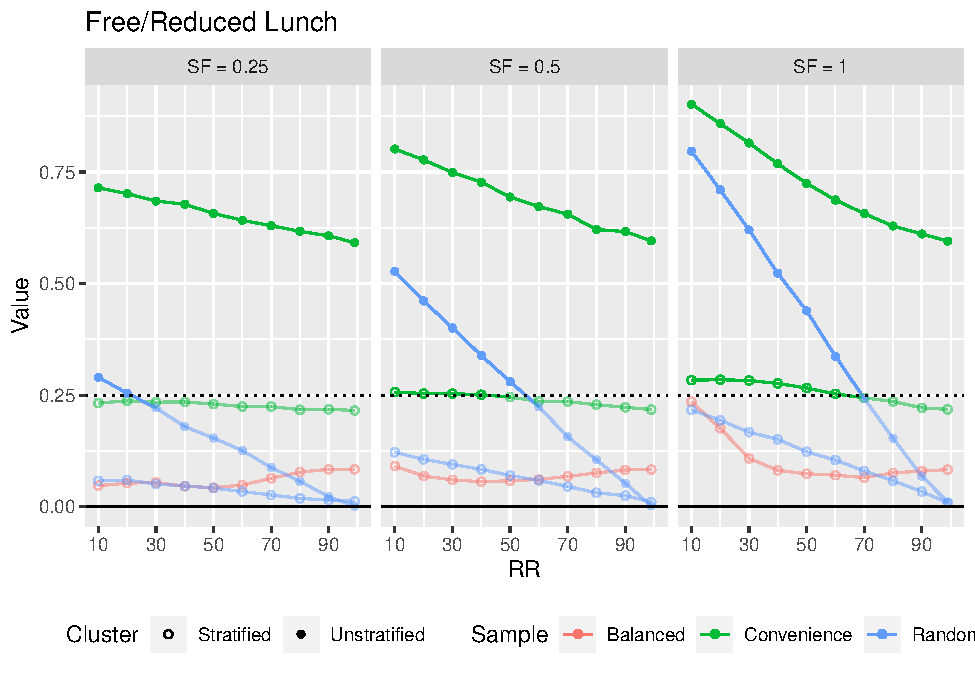
\includegraphics{5---Analysis_files/figure-latex/unnamed-chunk-21-1.pdf}

Analysis of Variance Table

Model 1: mSMD \textasciitilde{} RR
Model 2: mSMD \textasciitilde{} log\_odds + vratio + RR
Model 3: mSMD \textasciitilde{} log\_odds * vratio * RR
Res.Df RSS Df Sum of Sq F Pr(\textgreater F)\\
1 583 59.336\\
2 581 38.107 2 21.2295 196.574 \textless{} 2.2e-16 \textbf{\emph{
3 577 31.157 4 6.9494 32.174 \textless{} 2.2e-16 }}
---
Signif. codes: 0 \enquote{\emph{\textbf{' 0.001 '}' 0.01 '}} 0.05 \enquote{.} 0.1 ' ' 1

======================================================
Model 1 Model 2 Model 3\\
------------------------------------------------------
(Intercept) 0.24 *** 0.15 *** 0.11 *\\
(0.03) (0.03) (0.05)\\
RR -0.00 *** -0.00 *** -0.00\\
(0.00) (0.00) (0.00)\\
log\_odds 0.61 *** 1.24 \textbf{\emph{
(0.03) (0.16)\\
vratio 0.04 -0.02\\
(0.03) (0.08)\\
log\_odds:vratio -0.00\\
(0.28)\\
log\_odds:RR -0.02 }}
(0.00)\\
vratio:RR 0.00\\
(0.00)\\
log\_odds:vratio:RR 0.01\\
(0.00)\\
------------------------------------------------------
R\^{}2 0.04 0.39 0.50\\
Adj. R\^{}2 0.04 0.38 0.49\\
Num. obs. 585 585 585\\
======================================================
*** p \textless{} 0.001; ** p \textless{} 0.01; * p \textless{} 0.05

\begin{verbatim}
## `geom_smooth()` using method = 'loess' and formula 'y ~ x'
\end{verbatim}

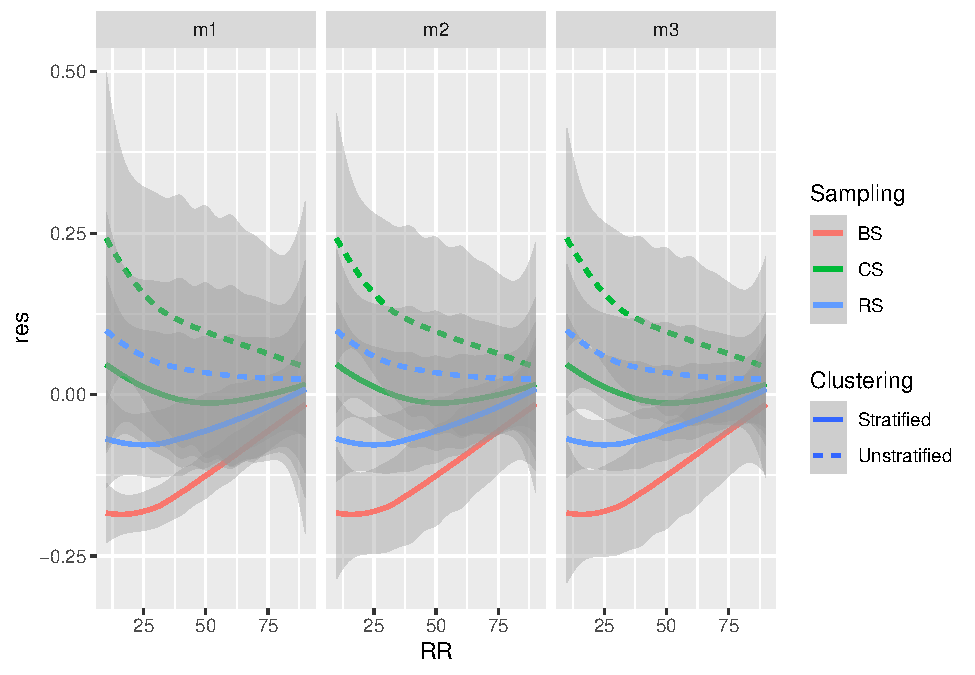
\includegraphics{5---Analysis_files/figure-latex/unnamed-chunk-22-1.pdf} 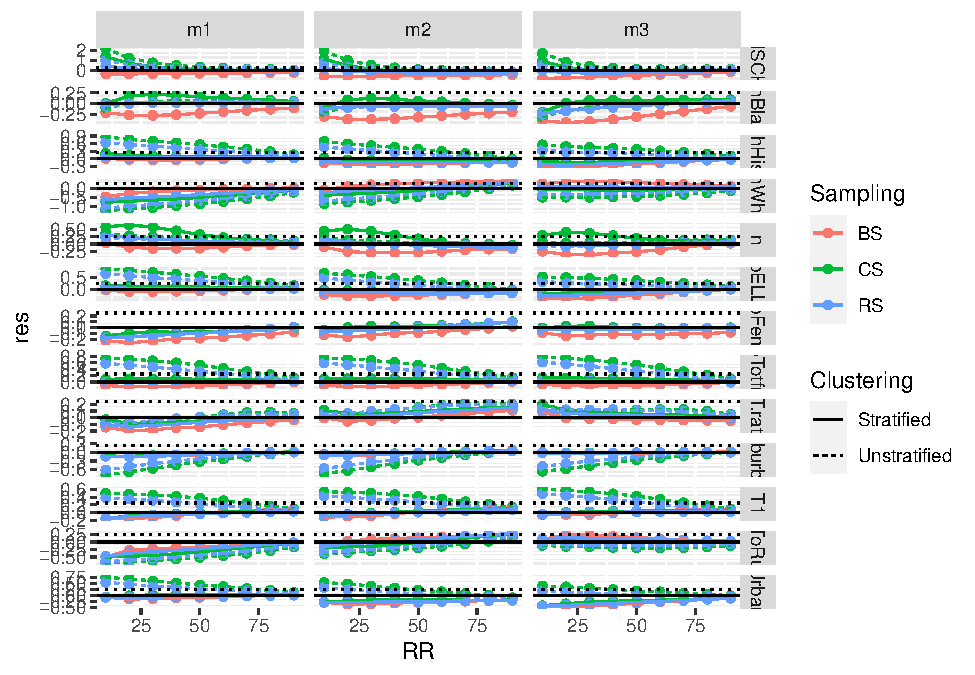
\includegraphics{5---Analysis_files/figure-latex/unnamed-chunk-22-2.pdf}

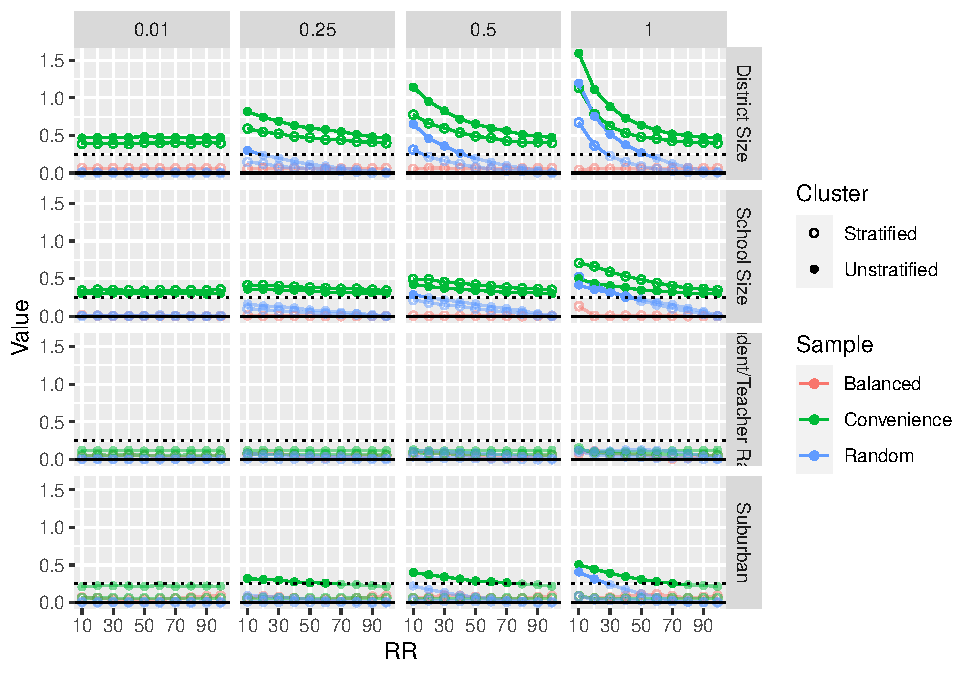
\includegraphics{5---Analysis_files/figure-latex/unnamed-chunk-23-1.pdf}
\#\#\# Test 2

\begin{verbatim}
## Joining, by = "var"
\end{verbatim}

\begin{verbatim}
## `summarise()` regrouping output by 'sample_method', 'RR', 'var', 'Sampling' (override with `.groups` argument)
\end{verbatim}

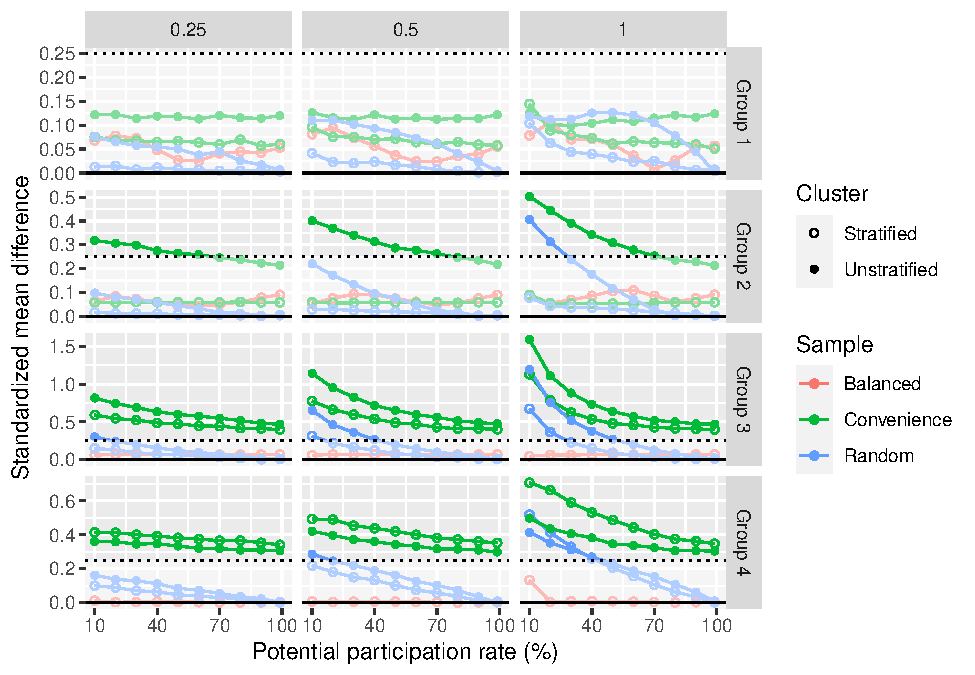
\includegraphics{5---Analysis_files/figure-latex/unnamed-chunk-24-1.pdf} 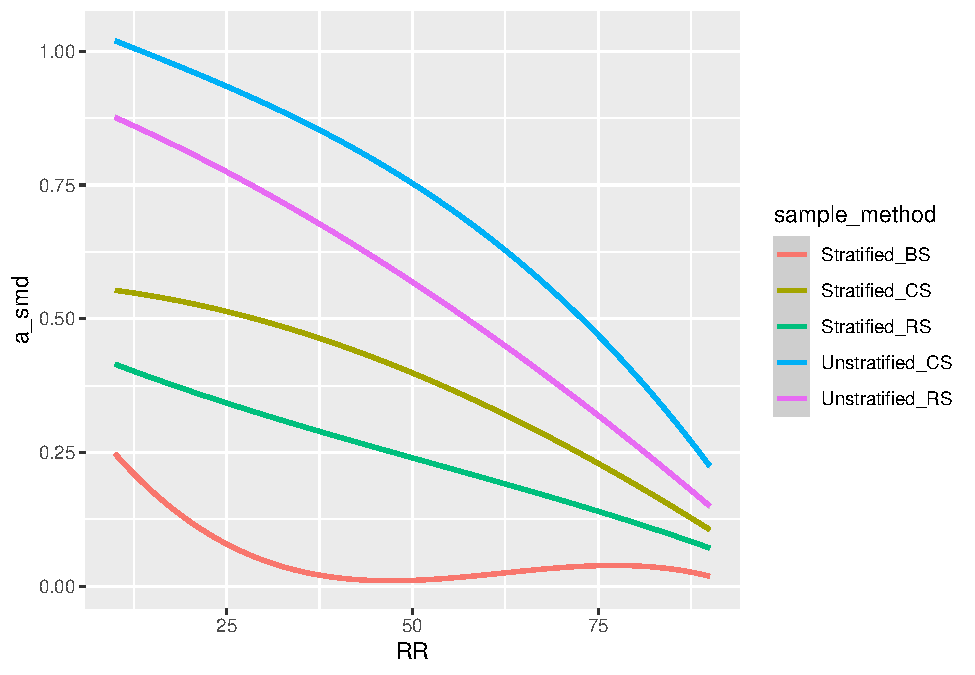
\includegraphics{5---Analysis_files/figure-latex/unnamed-chunk-24-2.pdf} 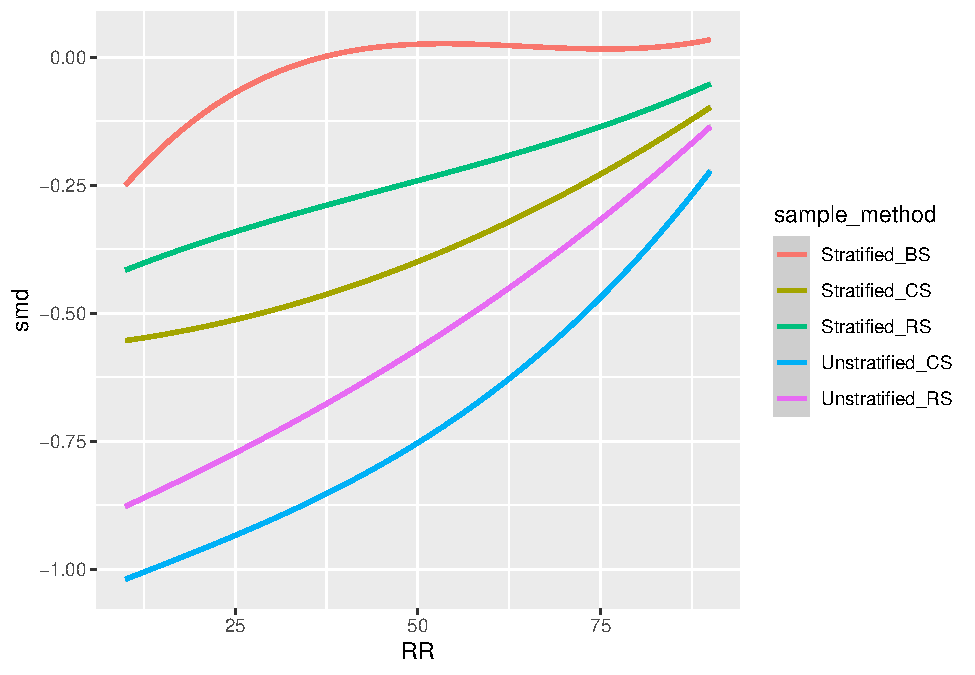
\includegraphics{5---Analysis_files/figure-latex/unnamed-chunk-24-3.pdf}

\hypertarget{feasibility}{%
\subsection{Feasibility}\label{feasibility}}

\hypertarget{sampling-difficulty}{%
\subsubsection{Sampling Difficulty}\label{sampling-difficulty}}

\begin{verbatim}
## `summarise()` regrouping output by 'sample_method', 'RR', 'measure', 'Sampling', 'Clustering' (override with `.groups` argument)
\end{verbatim}

\begin{figure}
\centering
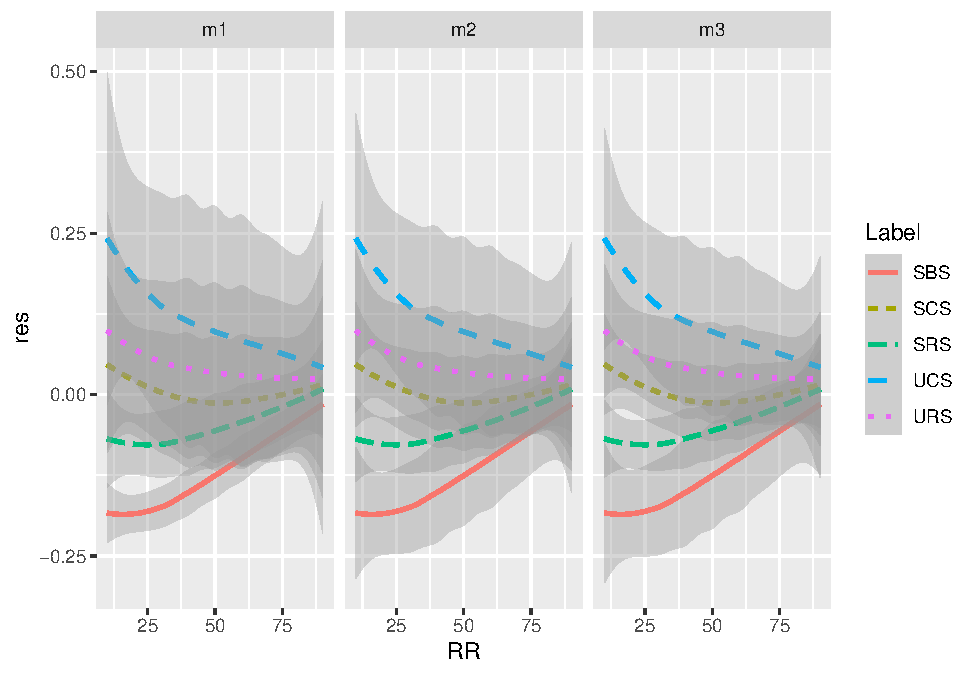
\includegraphics{5---Analysis_files/figure-latex/unnamed-chunk-27-1.pdf}
\caption{\label{fig:unnamed-chunk-27}Schools Contacted}
\end{figure}

\begin{figure}
\centering
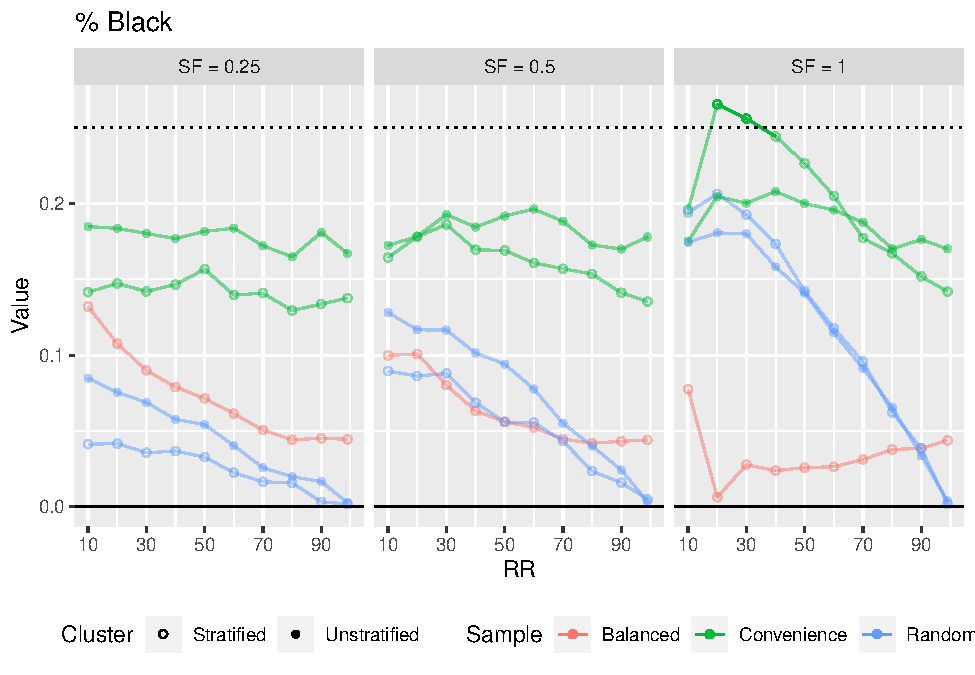
\includegraphics{5---Analysis_files/figure-latex/unnamed-chunk-28-1.pdf}
\caption{\label{fig:unnamed-chunk-28}Sampling response rates}
\end{figure}

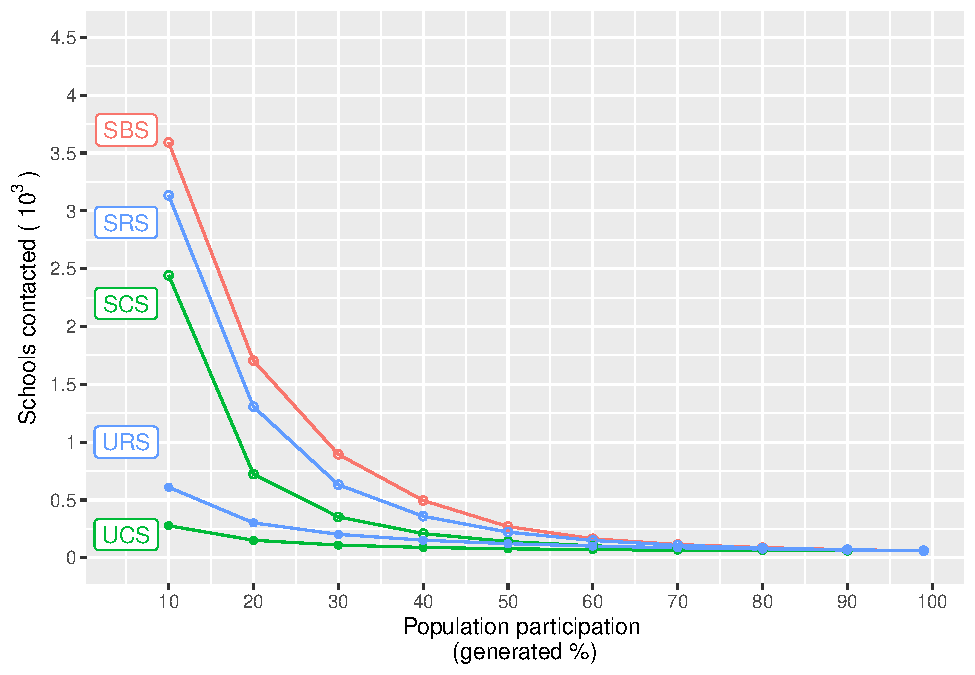
\includegraphics{5---Analysis_files/figure-latex/unnamed-chunk-29-1.pdf}

\hypertarget{relative-performance}{%
\subsubsection{Relative Performance}\label{relative-performance}}

\begin{verbatim}
## Joining, by = c("RR", "measure", "K")
\end{verbatim}

\hypertarget{gini-plot}{%
\subsubsection{Gini Plot}\label{gini-plot}}

\begin{verbatim}
## Joining, by = "DSID"
## Joining, by = "DSID"
## Joining, by = "DSID"
## Joining, by = "DSID"
## Joining, by = "DSID"
## Joining, by = "DSID"
## Joining, by = "DSID"
## Joining, by = "DSID"
## Joining, by = "DSID"
## Joining, by = "DSID"
## Joining, by = "DSID"
## Joining, by = "DSID"
## Joining, by = "DSID"
## Joining, by = "DSID"
## Joining, by = "DSID"
## Joining, by = "DSID"
## Joining, by = "DSID"
## Joining, by = "DSID"
## Joining, by = "DSID"
## Joining, by = "DSID"
## Joining, by = "DSID"
## Joining, by = "DSID"
## Joining, by = "DSID"
## Joining, by = "DSID"
## Joining, by = "DSID"
## Joining, by = "DSID"
## Joining, by = "DSID"
## Joining, by = "DSID"
## Joining, by = "DSID"
## Joining, by = "DSID"
## Joining, by = "DSID"
## Joining, by = "DSID"
## Joining, by = "DSID"
## Joining, by = "DSID"
## Joining, by = "DSID"
## Joining, by = "DSID"
## Joining, by = "DSID"
## Joining, by = "DSID"
## Joining, by = "DSID"
## Joining, by = "DSID"
## Joining, by = "DSID"
## Joining, by = "DSID"
## Joining, by = "DSID"
## Joining, by = "DSID"
## Joining, by = "DSID"
\end{verbatim}

\begin{verbatim}
## Warning: `cols` is now required when using unnest().
## Please use `cols = c(data)`
\end{verbatim}

\begin{verbatim}
## `summarise()` regrouping output by 'sample_method', 'Clustering', 'Sampling' (override with `.groups` argument)
\end{verbatim}

\hypertarget{export-plots}{%
\section{Export Plots}\label{export-plots}}


\end{document}
